\documentclass[border=10pt]{standalone}

\usepackage{tikz}
\usepackage{tikzsymbols}
\usetikzlibrary{calc,patterns,shapes.geometric}

\def\centerarc[#1](#2)(#3:#4:#5){\draw[#1] ($(#2)+({#5*cos(#3)},{#5*sin(#3)})$) arc (#3:#4:#5);}

\begin{document}
	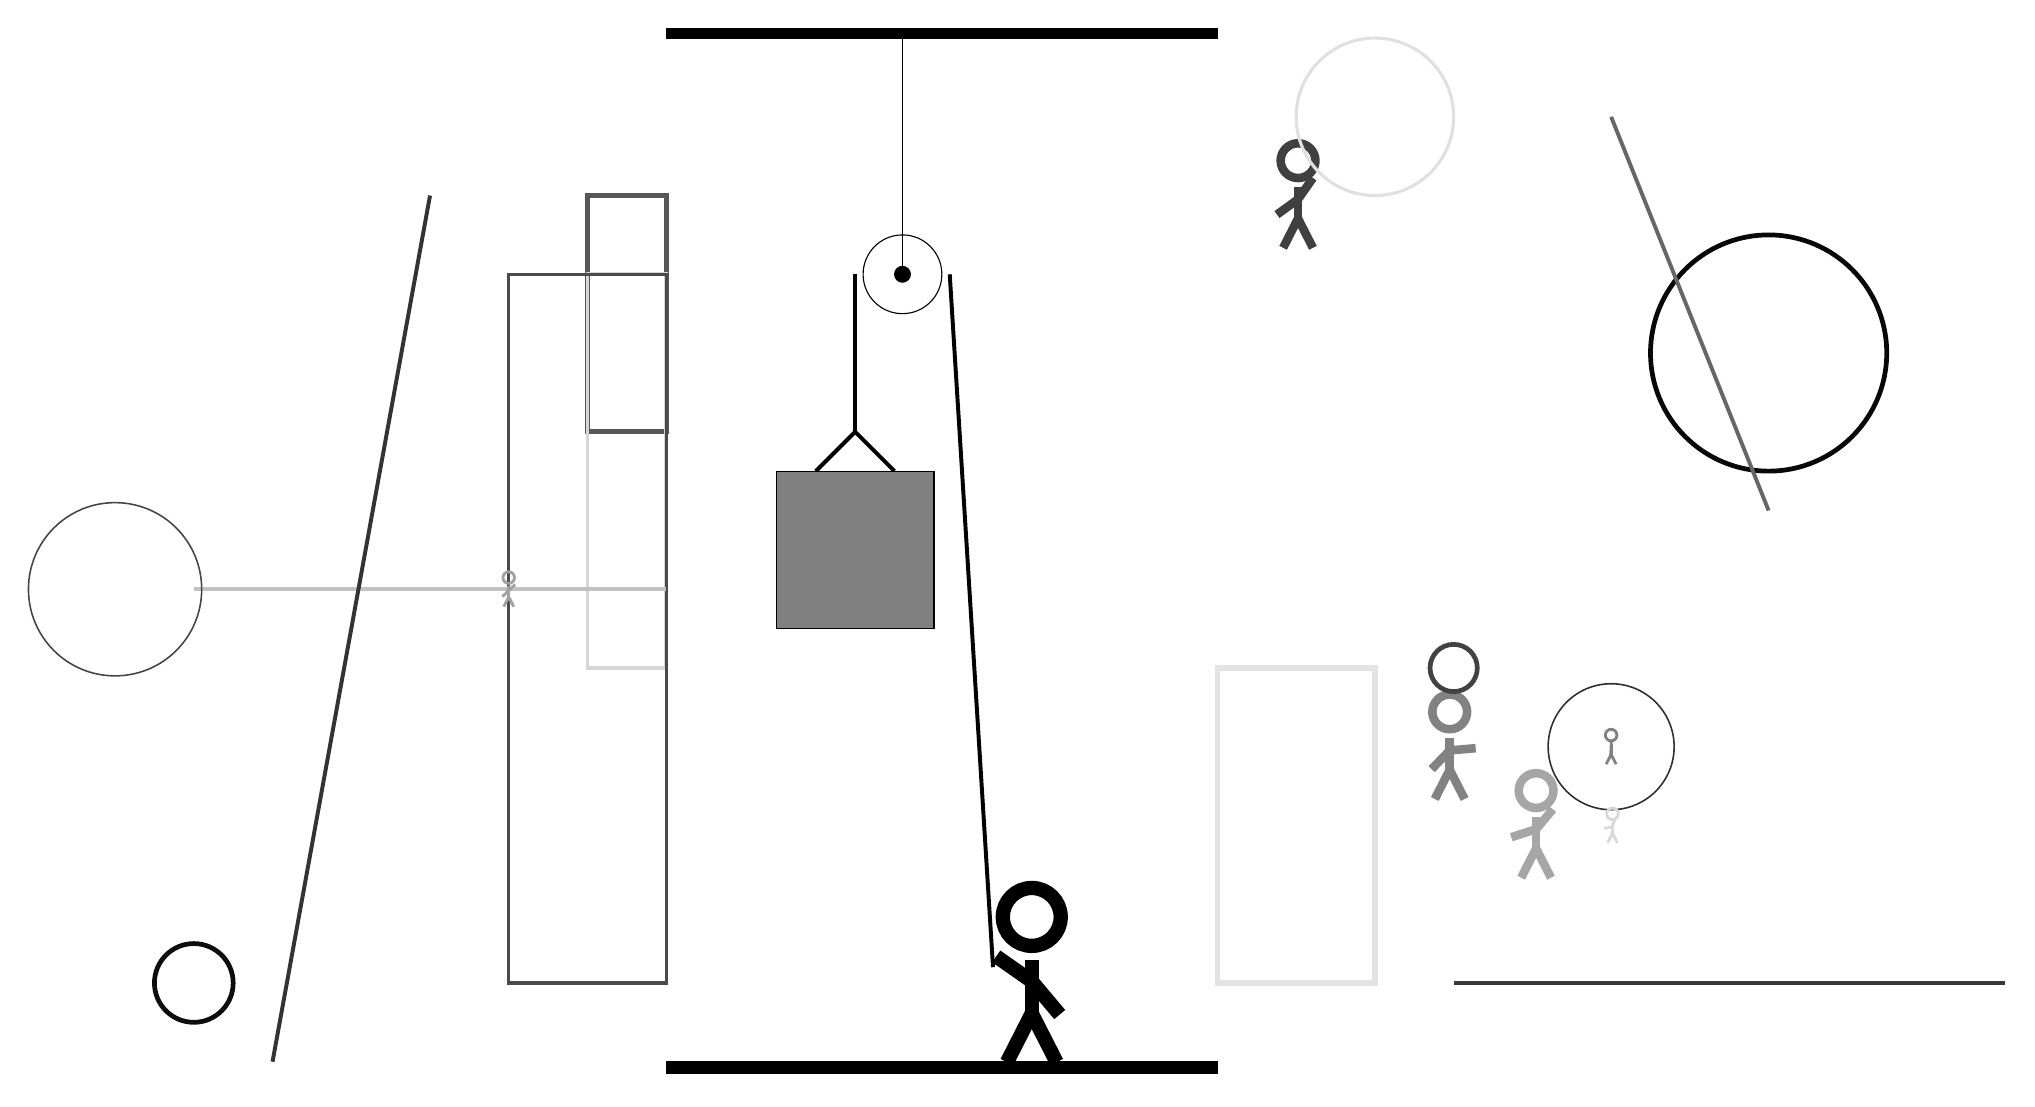
\begin{tikzpicture}
		%%%%% START %%%%%
		
		\draw[fill=black] (-2, 10) rectangle (5, 10.125);
		
		\draw[line width=0.6mm, color=black!66] (-3, 8) rectangle (-2, 5);
		
		\node[line width=0.7mm, color=black!75] at (6, 8) {\Strichmaxerl[6][36][55]};
		\draw[line width=0.5mm, color=black!16] (-3, 2) rectangle (-2, 7);
		\node[line width=0.7mm, color=black!49] at (10, 1) {\Strichmaxerl[2][86][89]};
		\node[line width=0.2mm, color=black!49] at (8, 1) {\Strichmaxerl[6][46][5]};
		
		\draw [line width=0.2mm, color=black!82](10, 1) circle (0.8);
		
		\draw [line width=0.6mm, color=black!95](-8, -2) circle (0.5);
		\draw[line width=0.4mm, color=black!71] (-2, -2) rectangle (-4, 7);
		\draw [line width=0.4mm, color=black!12](7, 9) circle (1.0);
		\draw[line width=0.5mm, color=black!24](-2, 3) -- (-8, 3);
		
		\node[line width=0.4mm, color=black!37] at (-4, 3) {\Strichmaxerl[2][44][43]};
		\node[line width=0.7mm, color=black!35] at (9, 0) {\Strichmaxerl[6][18][50]};
		\draw[line width=0.7mm, color=black!11] (7, -2) rectangle (5, 2);
		
		\node[line width=0.6mm, color=black!15] at (10, 0) {\Strichmaxerl[2][11][74]};
		\draw [line width=0.6mm, color=black!97](12, 6) circle (1.5);
		\draw[line width=0.5mm, color=black!60](10, 9) -- (12, 4);
		\draw [line width=0.2mm, color=black!73](-9, 3) circle (1.1);
		
		\draw[line width=0.5mm, color=black!78](8, -2) -- (15, -2);
		\draw[line width=0.5mm, color=black!80](-7, -3) -- (-5, 8);
		\draw [line width=0.6mm, color=black!74](8, 2) circle (0.3);
		
		\draw (1, 7) circle (0.5);
		\draw[fill=black] (1, 7) circle (0.1);
		\draw (1, 10) -- (1, 7);
		
		\draw[line width=0.5mm] (-0.1, 4.5) -- (0.4, 5.0) -- (0.9, 4.5);
		\draw[fill=black!50] (-0.6, 4.5) rectangle (1.4, 2.5);
		
		\draw[line width=0.5mm] (0.4, 7) -- (0.4, 5.0);
		\centerarc[line width=0.5mm](1, 7)(0:180:0.6);
		\draw[line width=0.5mm](1.6, 7) -- (2.15, -1.8);
		
		\node at (2.6, -1.9) {\Strichmaxerl[10][-35][-50]};
		
		\draw[fill=black] (-2, -3) rectangle (5, -3.15);
		
		%%%%% END %%%%%
	\end{tikzpicture}
\end{document}